\documentclass{beamer}

\mode<presentation>{
\usetheme{Madrid}
\setbeamertemplate{navigation symbols}{}
}

\usepackage{graphicx}
\usepackage{booktabs}
\usepackage[spanish]{babel}
\usepackage[latin1]{inputenc}

%====================================

\title[Trabajo de fin de m�ster]{Redes Generativas Antag�nicas}

\author[Ant�n Makarov]{Ant�n Makarov Samusev}
\institute[UCM/UPM]
{
Universidad Complutense de Madrid \\
\medskip
Universidad Polit�cnica de Madrid \\
\medskip
\textit{amakarov@ucm.es}
}
\date{25 de septiembre de 2019}

%====================================

\begin{document}

\begin{frame}
\titlepage
\end{frame}

%====================================

\begin{frame}
\frametitle{�ndice}
\tableofcontents
\end{frame}

%====================================

%------------------------------------------------
\section{Redes Generativas Antag�nicas}
%------------------------------------------------

\begin{frame}
	\frametitle{Descripci�n del problema}
	\begin{itemize}
	\item <1-> Goodfellow et. al. 2014
	\item <2-> Aprendizaje no supervisado
	\item <3-> Describir la distribuci�n que siguen los datos
	\item <4-> Generar muestras a partir de dicha distribuci�n
	\item <5->  Mediante redes neuronales que compiten entre s�
	\end{itemize}
\end{frame}

\begin{frame}
\frametitle{Idea conceptual}
\begin{figure}
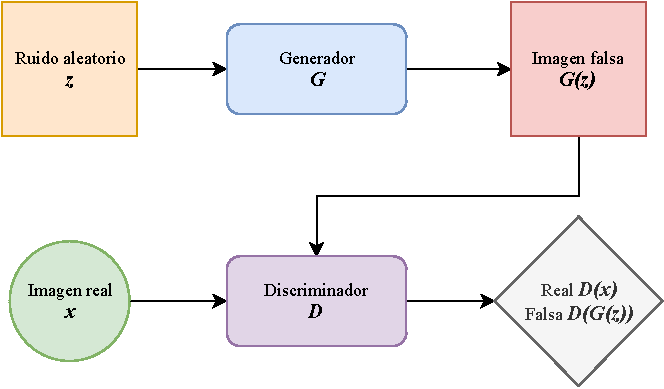
\includegraphics[width=0.8\linewidth]{../images/report/scheme.pdf}
\end{figure}
\end{frame}

\begin{frame}
\frametitle{Aspectos te�ricos}
\begin{equation*}
\min_G \max_D V(G,D) = \mathbb{E}_{x \sim p_d(x)} [\log D(x)] + \mathbb{E}_{z \sim p_z(z)} [\log (1- D(G(z)))].
\label{minimax}
\end{equation*}
\end{frame}

%------------------------------------------------
\section{Generaci�n de arte}
\subsection{DCGAN}
%------------------------------------------------

\begin{frame}
\frametitle{DCGAN}
\center \textbf{Deep Convolutional Generative Adversarial Network}
\vfill
\begin{itemize}
	\item 
\end{itemize}
\end{frame}

%------------------------------------------------
\subsection{Metodolog�a}
%------------------------------------------------

\begin{frame}
\frametitle{Obtenci�n y pre-procesado}
	\begin{itemize}
		\item Conjunto de datos obtenido en Kaggle
		\item M�s de 100000 im�genes $\approx 50$ GB
		\item Algunas im�genes corruptas
		\item Escalado de tama�os y proporciones
		\item Normalizaci�n
		\item Carga como tensores
	\end{itemize}
\end{frame}

\begin{frame}
	\frametitle{Arquitectura}
	\begin{figure}
		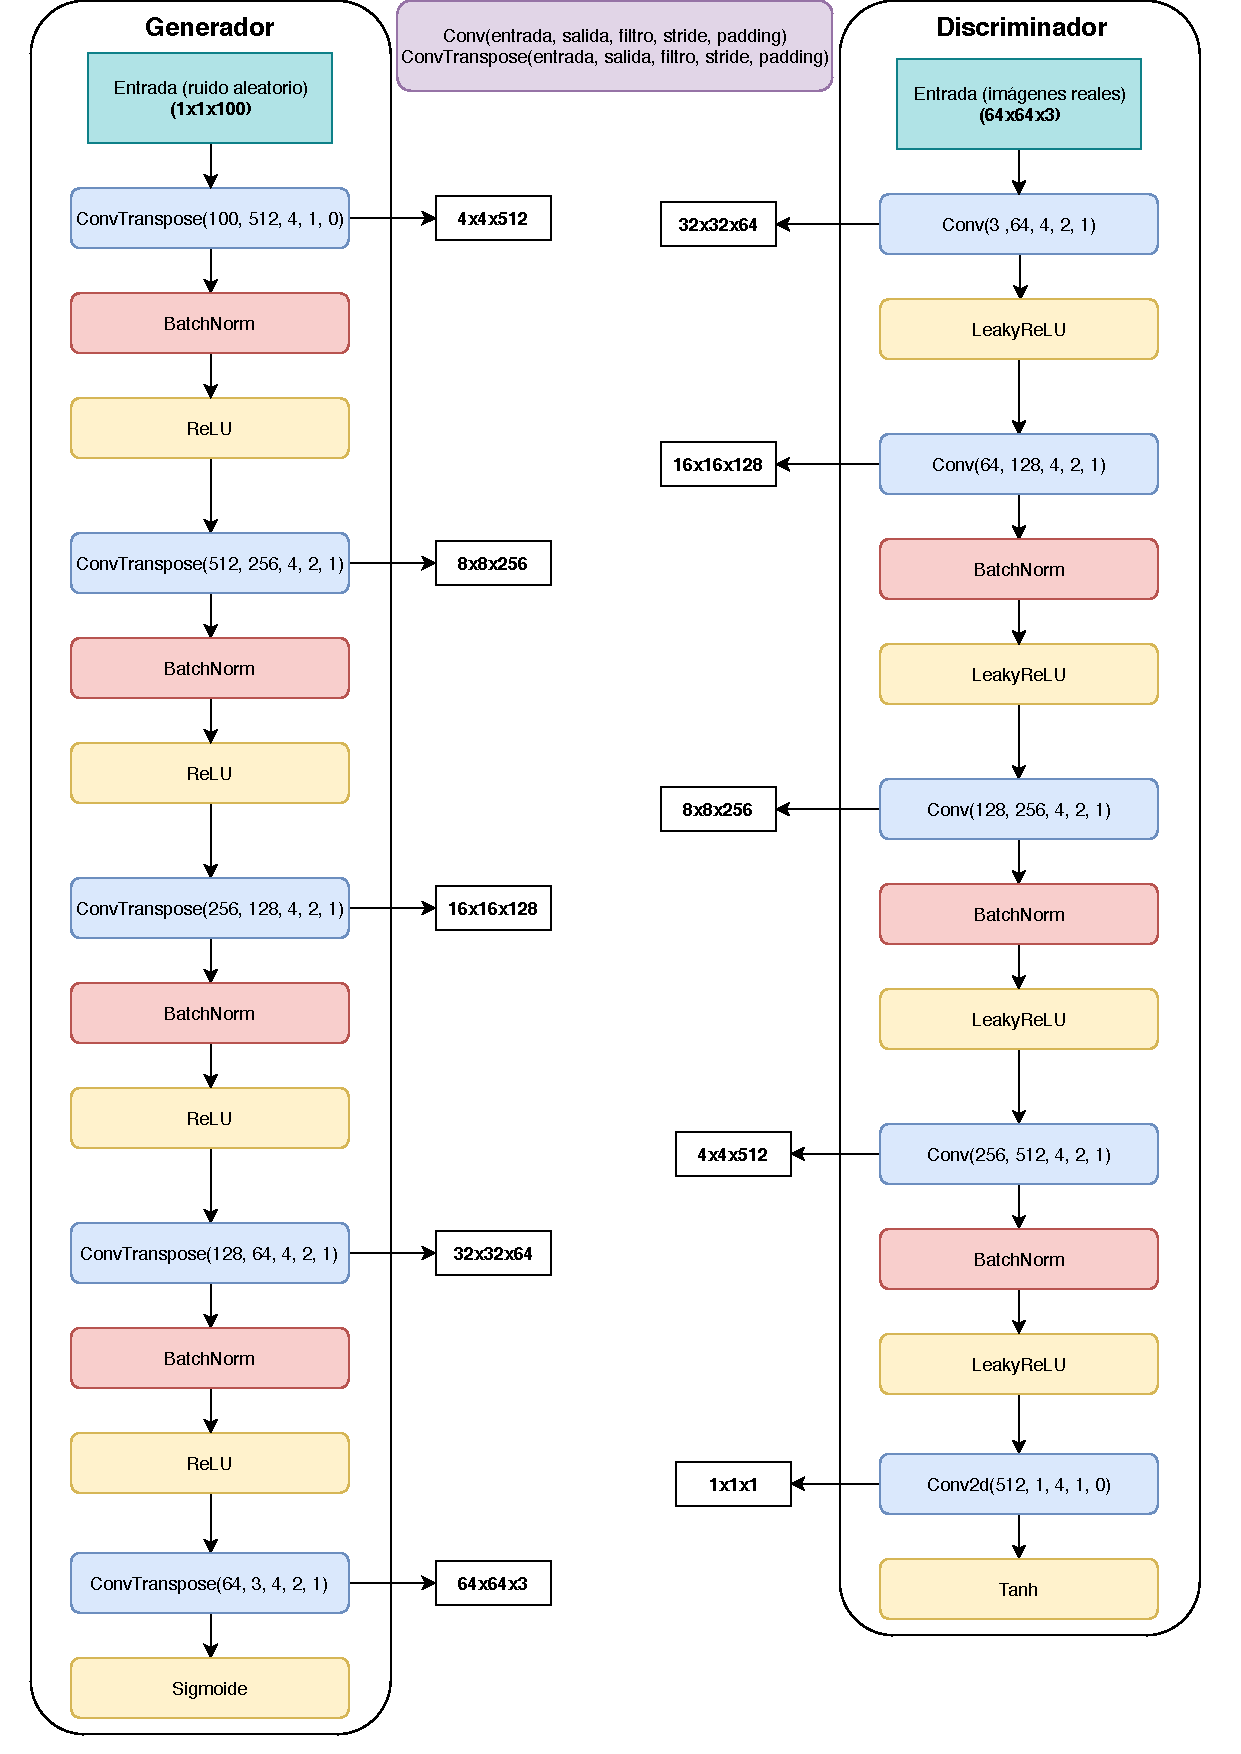
\includegraphics[width=0.45\linewidth]{../images/report/architecture.pdf}
	\end{figure}
\end{frame}

\begin{frame}
\begin{figure}
	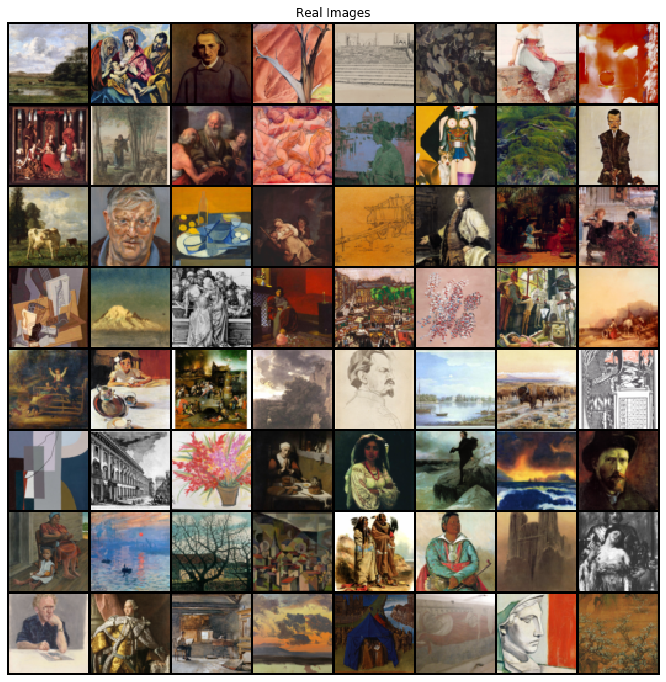
\includegraphics[width=0.7\linewidth]{../images/results/original_data.png}
\end{figure}
\end{frame}

%------------------------------------------------
\subsection{Resultados}
%------------------------------------------------

\begin{frame}
	\begin{figure}
		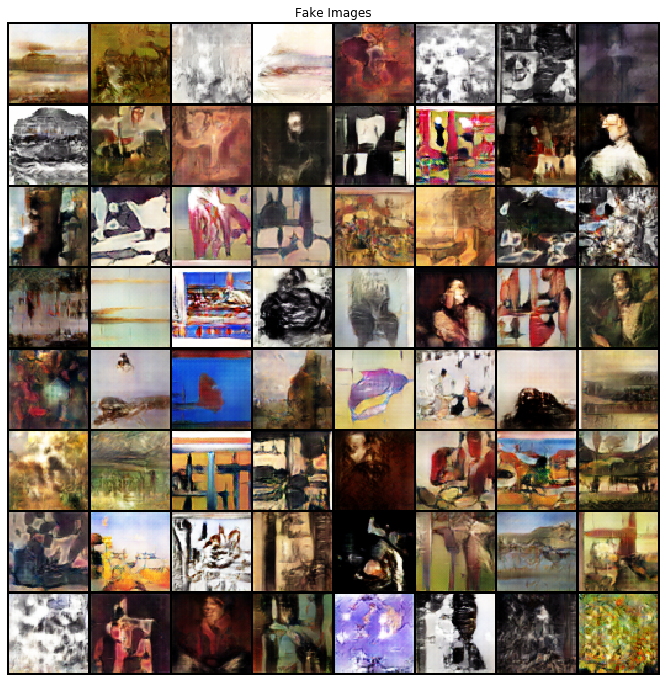
\includegraphics[width=0.7\linewidth]{../images/results/generated_data.png}
	\end{figure}
\end{frame}

%------------------------------------------------
\subsection{Recursos y rendimiento}
%------------------------------------------------

\begin{frame}
	\frametitle{Recursos y rendimiento}
	\begin{itemize}
		\item Imprescindible GPU para el entrenamiento
		\item 24 horas para 30 �pocas
		\item en PC normal, 20 veces m�s lento
	\end{itemize}
\end{frame}

%------------------------------------------------
\section{Arquitecturas basadas en GANs}
%------------------------------------------------

\begin{frame}
	\frametitle{Arquitecturas basadas en GANs}

\end{frame}

%------------------------------------------------
\section{Consideraciones pr�cticas}
%------------------------------------------------

\begin{frame}
	\frametitle{Consideraciones pr�cticas}
	\begin{itemize}
		\item �C�mo evaluar los resultados?
		\item �C�mo comparar arquitecturas?
		\item Mode collapse
	\end{itemize}
\end{frame}

%------------------------------------------------
\section{Conclusi�n}
%------------------------------------------------

\begin{frame}
\frametitle{Conclusi�n}
\begin{itemize}
	\item Campo de investigaci�n en auge
	\item 
\end{itemize}
\end{frame}

%------------------------------------------------
\section{Referencias principales}
%------------------------------------------------

\begin{frame}
\frametitle{Referencias principales}
\begin{thebibliography}{9}


\end{thebibliography}
\end{frame}

%------------------------------------------------

\begin{frame}
\centering
\Huge
Gracias por su atenci�n. \par
\vfill
�Preguntas?
\end{frame}

\end{document}